%%%%%%%%%%%%%%%%%%%%%%%%%%%%%%%%%%%%%
%                                   %
% Compile with XeLaTeX and biber    %
%                                   %
% Questions or comments:            %
%                                   %
% joshua dot mcneill at uga dot edu %
%                                   %
%%%%%%%%%%%%%%%%%%%%%%%%%%%%%%%%%%%%%

\documentclass{beamer}
  % Read in standard preamble (cosmetic stuff)
  %%%%%%%%%%%%%%%%%%%%%%%%%%%%%%%%%%%%%%%%%%%%%%%%%%%%%%%%%%%%%%%%
% This is a standard preamble used in for all slide documents. %
% It basically contains cosmetic settings.                     %
%                                                              %
% Joshua McNeill                                               %
% joshua dot mcneill at uga dot edu                            %
%%%%%%%%%%%%%%%%%%%%%%%%%%%%%%%%%%%%%%%%%%%%%%%%%%%%%%%%%%%%%%%%

% Beamer settings
% \usetheme{Berkeley}
\usetheme{CambridgeUS}
% \usecolortheme{dove}
% \usecolortheme{rose}
\usecolortheme{seagull}
\usefonttheme{professionalfonts}
\usefonttheme{serif}
\setbeamertemplate{bibliography item}{}

% Packages and settings
\usepackage{fontspec}
  \setmainfont{Charis SIL}
\usepackage{hyperref}
  \hypersetup{colorlinks=true,
              allcolors=blue}
\usepackage{graphicx}
  \graphicspath{{../../figures/}}
\usepackage[normalem]{ulem}
\usepackage{enumerate}

% Document information
\author{M. McNeill}
\title[FREN2001]{Français 2001}
\institute{\url{joshua.mcneill@uga.edu}}
\date{}

%% Custom commands
% Lexical items
\newcommand{\lexi}[1]{\textit{#1}}
% Gloss
\newcommand{\gloss}[1]{`#1'}
\newcommand{\tinygloss}[1]{{\tiny`#1'}}
% Orthographic representations
\newcommand{\orth}[1]{$\langle$#1$\rangle$}
% Utterances (pragmatics)
\newcommand{\uttr}[1]{`#1'}
% Sentences (pragmatics)
\newcommand{\sent}[1]{\textit{#1}}
% Base dir for definitions
\newcommand{\defs}{../definitions}


  % Packages and settings

  % Document information
  \subtitle[Étages et objets directs]{Les étages et les pronoms compléments d'objet direct}

\begin{document}
  % Read in the standard intro slides (title page and table of contents)
  \begin{frame}
    \titlepage
    \tiny{Office: % Basically a variable for office hours location
Gilbert 121\\
          Office hours: % Basically a variable for office hours
 lundi, mercredi, vendredi 10:10--11:10
}
  \end{frame}

  \begin{frame}{Cache-cache}
    \begin{columns}
      \column{0.5\textwidth}
        \scriptsize
        Cécile joue à cache-cache \gloss{hide-n-seek}.
        Est-ce qu'elle parle de son frère, sa sœur ou ses chats?
        \begin{enumerate}
          \item Elle les cherche dans la cour.
          \item<2->[$\to$] Ses chats.
          \item<3-> Elle le cherche dans la rue.
          \item<4->[$\to$] Son frère.
          \item<5-> Une femme au deuxième étage la voit sur le trottoir.
          \item<6->[$\to$] Sa sœur.
          \item<7-> Cécile veut les trouver au rez-de-chaussée.
          \item<8->[$\to$] Ses chats.
          \item<9-> La femme dit: <<Alors, prenez-la plus tard dans le bâtiment.>>
          \item<10->[$\to$] Sa sœur.
          \item<11-> Cécile dit: <<Ne le cherche pas dans la voiture dans le garage.>>
          \item<12->[$\to$] Son frère.
        \end{enumerate}
      \column{0.5\textwidth}
        \begin{minipage}[t][0.6\textheight]{\linewidth}
          \begin{center}
            \only<1-2>{
              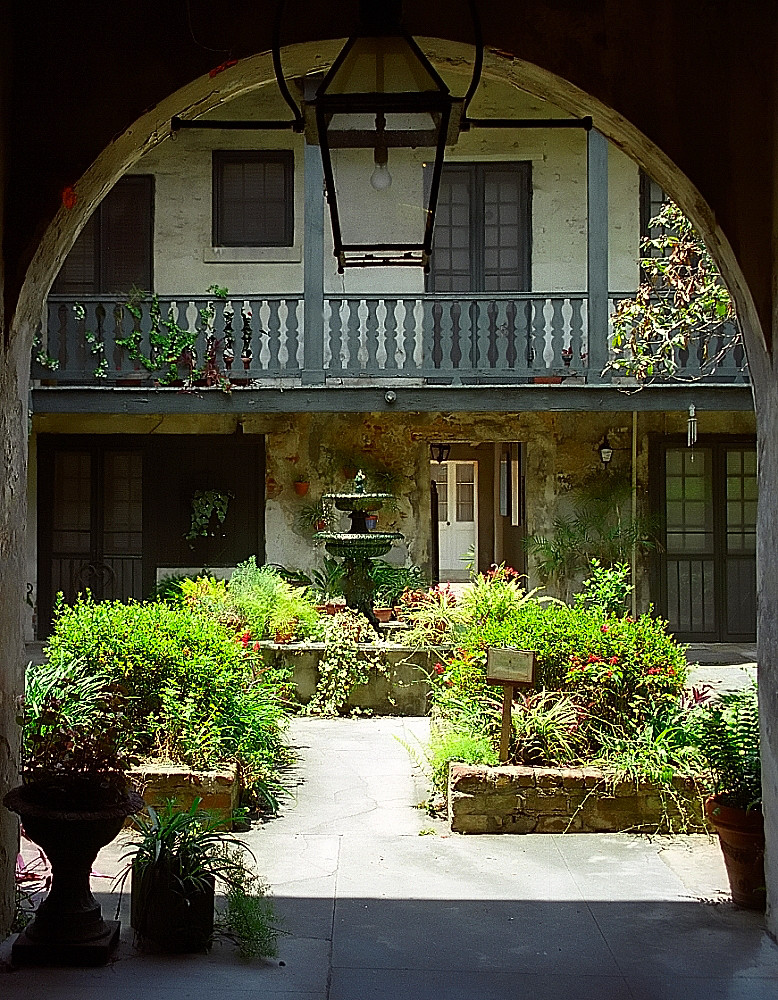
\includegraphics[scale=0.18]{cour.jpg}
            }
            \only<3-10>{
              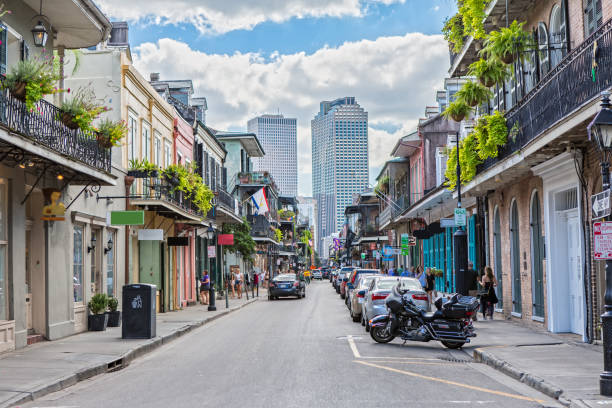
\includegraphics[scale=1.15]{rue.jpg}
            }
            \only<11-12>{
              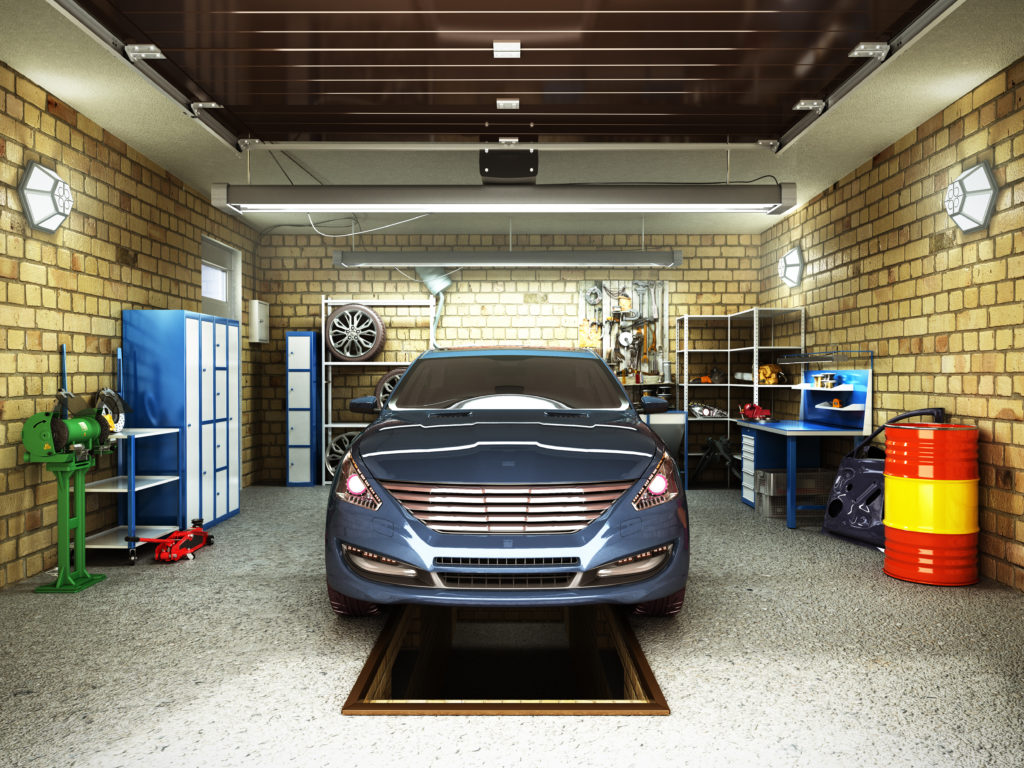
\includegraphics[scale=0.7]{garage.jpg}
            }
          \end{center}
        \end{minipage}
    \end{columns}
  \end{frame}

  \begin{frame}{}
    \begin{center}
      \Large Quiz
    \end{center}
  \end{frame}

  \begin{frame}{Est-ce que tu le choisis?}
    \small
    En groupes de trois ou quatre, expliquez pourquoi vous choisissez la chose mentionnée ou non.
    \begin{description}
      \item[\textbf{Modèle:}] \emph{un très petit appartement au cinquième étage dans une grande ville}
      \item[E1:] Je le choisis parce que j'aime être près des magasins et des restaurants.
      \item[E2:] Pas moi! Je ne le choisis pas. Je veux une grande maison avec un garage.
    \end{description}
    \begin{enumerate}
      \item un très petit appartement au cinquième étage dans une grande ville
      \item une grande salle de séjour dans une vieille maison
      \item un très beau appartement au quatrième mais sans ascenseur
      \item un jardin avec beaucoup de fleurs
      \item un studio chic au rez-de-chaussée en centre-ville
    \end{enumerate}
  \end{frame}

  \begin{frame}{Vous êtes d'accord?}
    Avec un/e partenaire, décidez si vous êtes d'accord ou non la phrase.
    \begin{description}
      \item[\textbf{Modèle:}] \emph{On les aime, les films?}
      \item[E1:] Oui, je les aime. Je vais à Ciné en centre-ville pour les regarder.
      \item[E2:] Moi, je ne les aime pas.
    \end{description}
    \begin{columns}[t]
      \column{0.5\textwidth}
        \begin{enumerate}
          \item On l'aime beaucoup, le théâtre?
          \item On l'aime bien, le coca?
          \item On les écoute toujours, les parents?
          \item On les déteste, les essais?
        \end{enumerate}
      \column{0.5\textwidth} 
        \begin{enumerate}
          \setcounter{enumi}{4}
          \item On les regarde souvent, les documentaires?
          \item On le visite souvent, le musée?
          \item On l'adore, la philosophie?
          \item On les aime, les cours?
        \end{enumerate}
    \end{columns}
  \end{frame}

  \begin{frame}{}
    \begin{center}
      \Large Questions?
    \end{center}
  \end{frame}
\end{document}
